\documentclass{../lista}

\begin{document}
	\cabecalho{2}{Questões}{Mecânica Celeste}{Iago Mendes}

	\begin{questao}{1 ponto}
		Medir distâncias sempre foi uma tarefa importante dentro da Astronomia e um dos métodos mais simples e conhecidos é o uso da paralaxe ($\pi$), que nada mais é do que uma medida de ângulo feita ao longo da translação terrestre ao redor do Sol. Observe o esquema a seguir:
		\begin{figure}[H]
			\centering
			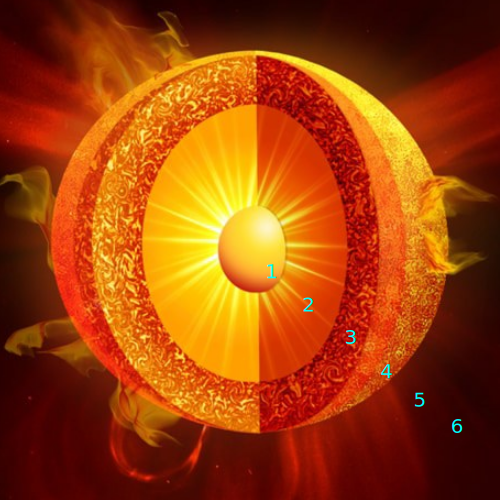
\includegraphics[scale=0.7]{./img/1.png}
		\end{figure}
		Ele representa como é possível medir a paralaxe ($\pi$), por meio da medição do deslocamento angular da estrela em relação às estrelas de fundo (as quais podemos consider como fixas na Esfera Celeste neste caso) durante um período de tempo $\Delta t$ que a Terra leva para ir de $T_1$ para $T_2$ (posições na órbita terrestre). No esquema, $R_T$ é o raio orbital da terra ($R_T = 1 \; UA \textrm{ (unidade astronômica)} \simeq 1.5 \cdot 10^{11} \; m$) e $r$ é a distância da estrela, a qual queremos determinar.

		\begin{pergunta}{0,25 ponto}
			Qual o valor aproximado de $\Delta t$ de acordo com o esquema?

			\begin{alternativas}
				\item $365,25$ dias
				\item $182,625$ dias
				\item $23h \, 56min$
				\item $11h \, 58min$
			\end{alternativas}
		\end{pergunta}

		\begin{pergunta}{0,25 ponto}
			Desenvolva uma fórmula para calcular $r$ a partir de $R_T$ e $\pi$.

			\espacoCalculo
			\espacoRespostaPergunta
		\end{pergunta}

		\begin{pergunta}{0,25 ponto}
			Sabendo que $1 \; pc \simeq 206.265 \; UA$, melhore a fórmula encontrada na pergunta anterior para que $r$ seja dado em parsecs ($pc$) e $\pi$ em segundos de arco ($''$). \\
			Dica: substitua o valor de $R_T$.

			\espacoCalculo[12cm]
			\espacoRespostaPergunta
		\end{pergunta}

		\begin{pergunta}{0,25 ponto}
			Sirius -- a estrela mais brilhante da esfera celeste -- possui uma paralaxe de $0.379''$. Qual a sua distância até a Terra em parsecs? \\
			Observação: sua resposta deve conter pelo menos 2 casas decimais.

			\espacoCalculo
			\espacoRespostaPergunta
		\end{pergunta}
	\end{questao}

	\begin{questao}{1 ponto}
		A energia mecânica ($E$) de um corpo em órbita é dada pela soma da energia cinética ($K$) e da energia gravitacional ($U$). Ou seja:
		\begin{equation}
			E=K+U
		\end{equation}

		\begin{pergunta}{0,5 ponto}
			Um corpo orbitante atinge a velocidade de escape ($v_{esc}$) quando $E=0$. Sabendo disso, encontre a fórmula de $v_{esc}$. \\
			Dica: $U = - \frac{GMm}{r}$, em que $G$ é a constante gravitacional, $M$ e $m$ são massas de 2 corpos (considere que $m$ orbita $M$), e $r$ é a distância de $m$ até $M$.

			\espacoCalculo[10cm]
			\espacoRespostaPergunta
		\end{pergunta}

		\begin{pergunta}{0,5 ponto}
			A partir de conceitos mais avançados, é possível encontrar a seguinte fórmula para $E$:
			\begin{equation}
				E = -\frac{GMm}{2a}
			\end{equation}
			em que $a$ é o semi-eixo maior da órbita. Comparando as 2 equações de $E$ mostradas nesta questão, encontre a fórmula da velocidade orbital $v$ de $m$ a qualquer distância $r$ de $M$.

			\espacoCalculo[10cm]
			\espacoRespostaPergunta
		\end{pergunta}
	\end{questao}

	\begin{questao}{1 ponto}
		Devido ao esforço de Loinha -- estudante apresentada na 1ª lista -- nas Seletivas Online, ela foi aceita para as Seletivas Presenciais, em Barra do Piraí-RJ. Enquanto ela estava aprofundando seus estudos em Mecânica Celeste, achou interessante o tópico de Pontos Lagrangianos e decidiu fazer uma maquete do Sistema Solar ressaltando os Objetos Troianos na órbita de Júpiter. \\
		Contudo, antes de fazer a maquete, Loinha desenhou o seguinte esquema para poder entender um pouco mais sobre esse tópico:
		\begin{figure}[H]
			\centering
			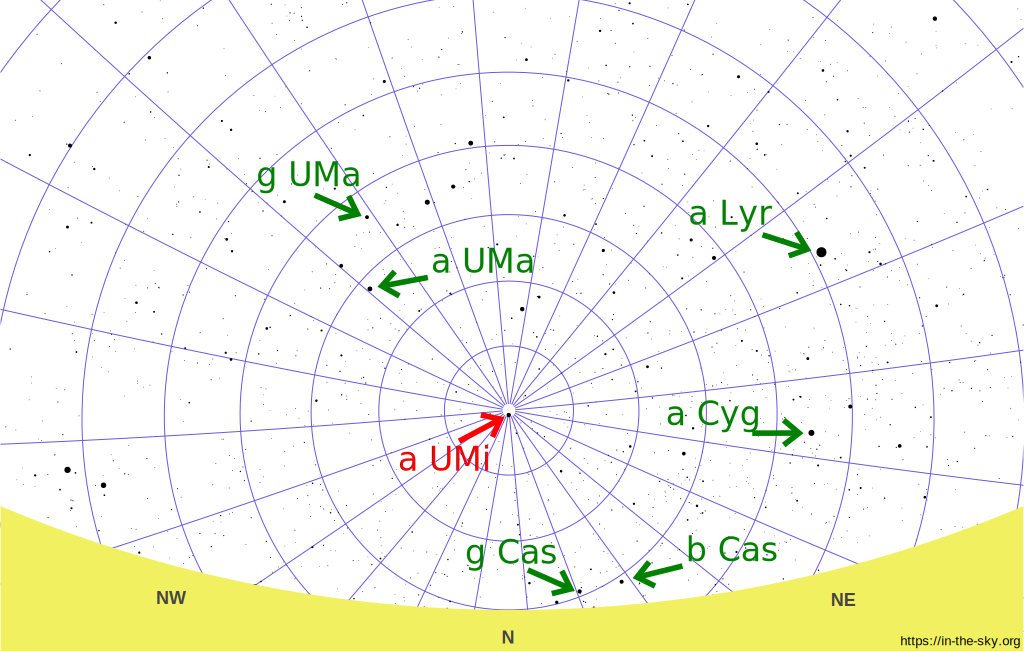
\includegraphics[scale=0.5]{./img/3.png}
		\end{figure}
		Além disso, Loinha anotou em seu caderno que os pontos $L_1$, $L_2$ e $L_3$ são instáveis gravitacionalmente, enquanto que os pontos $L_4$ e $L_5$ são estáveis.

		\begin{pergunta}{0,25 ponto}
			O que os Pontos de Lagrange possuem em comum?
			\begin{alternativas}
				\item Período orbital
				\item Semi-eixo maior
				\item Semi-eixo menor 
			\end{alternativas}
		\end{pergunta}

		\begin{pergunta}{0,25 ponto}
			Em qual categoria os Objetos Troianos podem ser classificados?
			\begin{alternativas}
				\item Planetas
				\item Planetas anões
				\item Cometas
				\item Asteroides
			\end{alternativas}
		\end{pergunta}

		\begin{pergunta}{0,5 ponto}
			Em qual(s) Ponto(s) Lagrangiano(s) Loinha deve colocar os Objetos Troianos na órbita de Júpiter para que a maquete seja mais realista?
			\begin{alternativas}
				\item $L_1$
				\item $L_2$
				\item $L_3$
				\item $L_4$
				\item $L_5$
			\end{alternativas}
		\end{pergunta}
	\end{questao}

	\begin{questao}{1 ponto}
		Em 2020, foi relavada a descoberta do exoplaneta \textit{AU Microscopii b}, o qual foi observado pelo \textit{Transiting Exoplanet Survey Satellite (TESS)} por meio do método de trânsito. Observe uma simulação disponível \href{https://exoplanets.nasa.gov/exoplanet-catalog/7635/au-microscopii-b/}{neste site}, a qual mostra o planeta orbitando a sua estrela (\textit{AU Microscopii}):
		\begin{figure}[H]
			\centering
			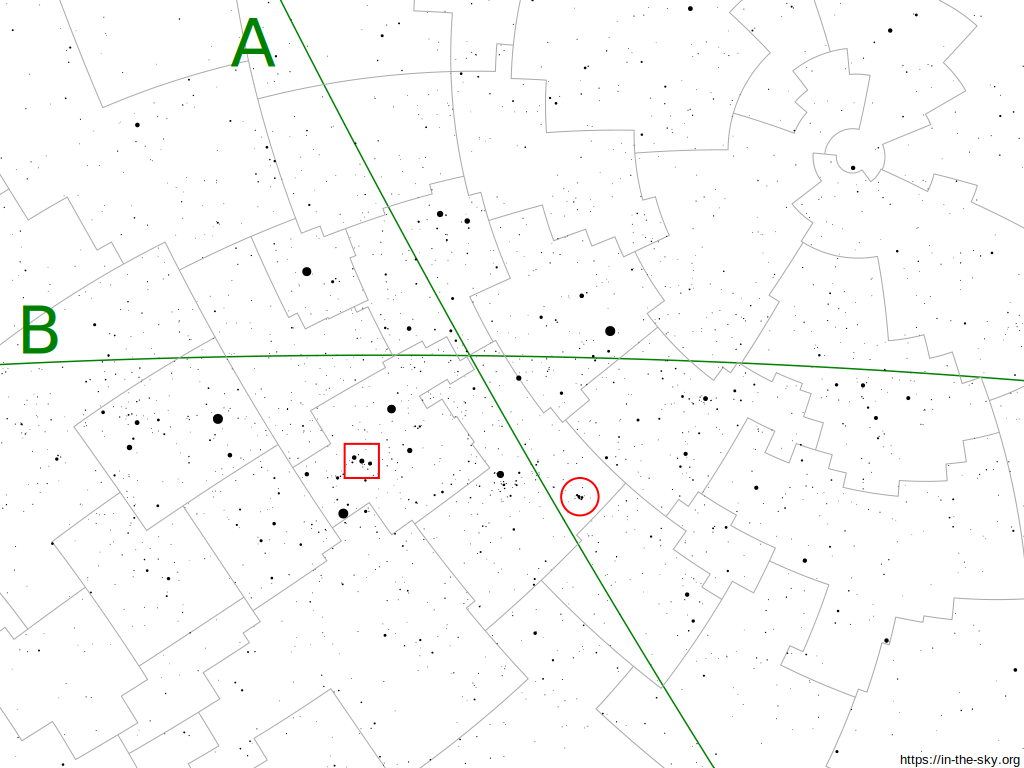
\includegraphics[scale=0.5]{./img/4.png}
		\end{figure}

		\begin{pergunta}{0,5 ponto}
			Com os dados a seguir (simplificados para facilitar as contas), calcule a massa da estrela \textit{AU Microscopii}. \\
			\textbf{Dados:}
				\begin{itemize}
					\item[$>$] Período orbital do exoplaneta: $T = 8,5 \; \textrm{dias} = 3,06 \cdot 10^4 \; s \approx 3 \cdot 10^4 \; s$
					\item[$>$] Raio orbital do exoplaneta: $r = 0,066 \; UA \simeq 9,87 \cdot 10^9 \; m \approx 1 \cdot 10^{10} \; m$
					\item[$>$] Constante gravitacional: $G \simeq 6,67 \cdot 10^{-11} \; \frac{m^3}{kg \, s^2} \approx 7 \cdot 10^{-7} \; \frac{m^3}{kg \, s^2}$
					\item[$>$] Aproximação de pi: $\pi \approx 3$
				\end{itemize}
			\textbf{Dica:} na 3ª Lei de Kepler desenvolvida, a constante de proporcionalidade pode ser calculada da seguinte forma:
				\begin{equation}
					k = \frac{4 \pi^2}{G(M+m)} \simeq \frac{4 \pi^2}{GM} \quad \leftrightarrow \quad M>>m
				\end{equation}
			
			\espacoCalculo[7cm]
			\espacoRespostaPergunta
		\end{pergunta}

		\begin{pergunta}{0,5 ponto}
			Com os seguintes dados, encontre a razão entre as constantes $k_M$ (sistema estelar de \textit{AU Microscopii}) e $k_S$ (sistema solar). \\
			\textbf{Dados:}
				\begin{itemize}
					\item[$>$] Período orbital da Terra: $T \simeq 3,15 \cdot 10^7 \; s \approx 3 \cdot 10^7 \; s$
					\item[$>$] Raio orbital da Terra: $r = 1 \; UA \simeq 1,5 \cdot 10^{11} \; m$
					\item[$>$] Massa do Sol: $M \simeq 2 \cdot 10^{30} \; kg$
				\end{itemize}
			
			\espacoCalculo[7cm]
			\espacoRespostaPergunta
		\end{pergunta}
	\end{questao}

	\begin{questao}{1 ponto}
		Apesar de a nossa estrela -- o Sol -- ser solitária, é comum encontrar sistemas estelares com 2 ou até mesmo mais componentes. Em um sistema binário, de acordo com a relação das massas, a massa e a distância ao baricentro (centro de massa) são inversalmente proporcionais, ou seja:
		\begin{equation}
			m_Ar_A=m_Br_B
		\end{equation}
		Além disso, geralmente é útil utilizarmos uma simplificação da 3ª Lei de Kepler, em que conseguimos retirar as constantes ao usar unidades astronômicas ($UA$) para $r$ ($r=r_A+r_B$), anos terrestres ($a$) para $T$, e massas solares ($M_{Sol}$) para $M$ ($M=m_A+m_B$). Com isso, temos a seguinte equação:
		\begin{equation}
			\frac{r^3}{T^2}=M
		\end{equation}
		Por fim, vale lembrar da Lei da Gravitação Universal, desenvolvida por Newton, a qual estabelece uma fórmula para a força gravitacional:
		\begin{equation}
			| F_g | = \frac{Gm_Am_B}{r^2}
		\end{equation}
		Dito isso, considere o esquema de um sistema binário a seguir:
		\begin{figure}[H]
			\centering
			\includegraphics[scale=0.4]{./img/5.png}
		\end{figure}
		em que $A$ e $B$ são 2 estrelas conectadas gravitacionalmente, e $r_A$ e $r_B$ são as suas respectivas distâncias ao centro de massa.

		\begin{pergunta}{0,1 ponto}
			Se $m_A=m_B= 5 \; M_{Sol}$ e $r_A=2 \; UA$, qual o valor de $r_B$?

			\espacoCalculo
			\espacoRespostaPergunta
		\end{pergunta}

		\begin{pergunta}{0,4 ponto}
			Calcule o valor de $T$ em anos terrestres.
			
			\espacoCalculo[7cm]
			\espacoRespostaPergunta
		\end{pergunta}

		\begin{pergunta}{0,5 ponto}
			Calcule o módulo da força gravitacional entre $A$ e $B$ em newtons. \\
			\textbf{Dados:}
				\begin{itemize}
					\item[$>$] Massa solar: $M_{Sol} \simeq 2 \cdot 10^{30}$
					\item[$>$] Unidade astronômica: $1 \; UA \simeq 1,5 \cdot 10^{11} \; m$
					\item[$>$] Constante gravitacional: $G \simeq 6,67 \cdot 10^{-11} \; \frac{m^3}{kg \, s^2} \approx 7 \cdot 10^{-7} \; \frac{m^3}{kg \, s^2}$
				\end{itemize}
			
			\espacoCalculo[7cm]
			\espacoRespostaPergunta
		\end{pergunta}
	\end{questao}
	
	\encerramento
\end{document}